We hire crowd workers on Prolific to evaluate the correctness of model-generated reasoning chains that result in a correct answer. We sample 100 reasoning chains for each domain generated by \texttt{code-davinci-002} with the greedy decoding strategy, where each set of 100 contains an equal number of samples from all datasets within the domain. We further require annotators to have experience coding in the programming language of the dataset they annotate (Python for MWP/CLUTRR/Sports/Date, and Scala for StrategyQA, as Datalog was not an option in Prolific). We have a single survey for each domain, with the exception of Multi-hop QA (in this case, we have separate surveys for StrategyQA, Date, and Sports, given the different nature of each dataset). Additionally, there was no way to ensure annotators knew PPDL on Prolific. In order to ensure high-quality annotations for SayCan, the authors annotate this dataset themselves. 

\begin{figure}
    \centering
    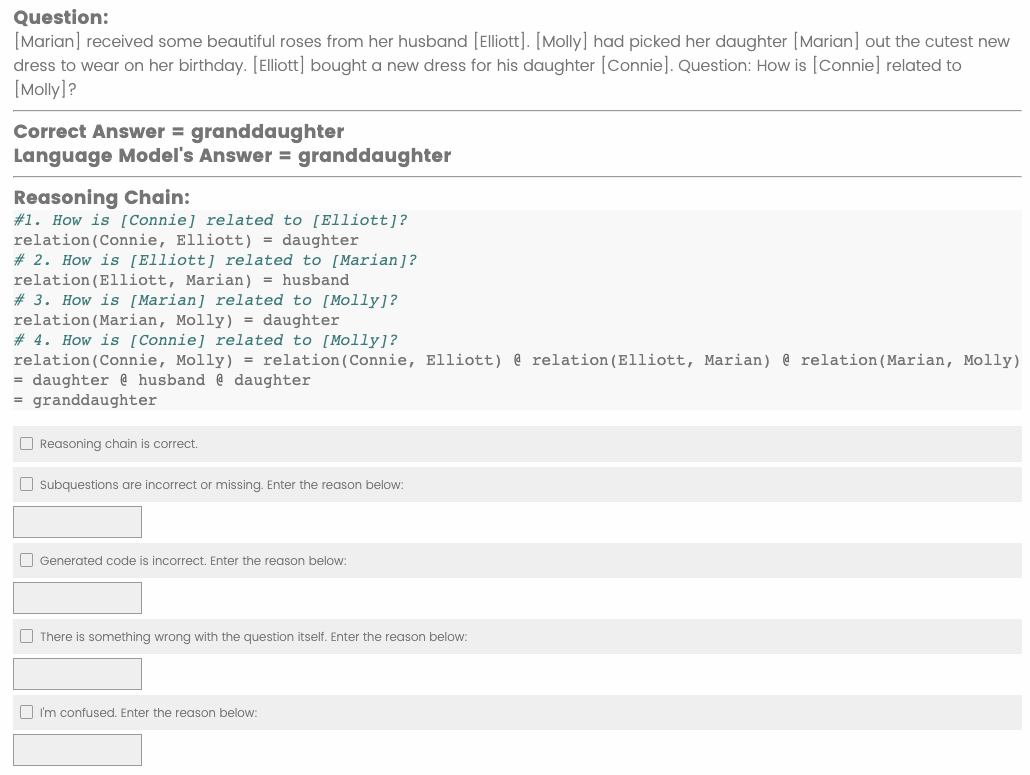
\includegraphics[width=\linewidth]{img/human_study_interface.png}
    \caption{Example of our annotation interface for the CLUTRR survey.}
    \label{fig:interface}
\end{figure}


\begin{table*}[h]
    \centering
    \vskip 0.15in
    \small
    \begin{tabular}{lrrrrr|r}
         \toprule
         Domain &  Correct & Incorrect NL & Incorrect SL & Flawed Question & Confused & Agreement\\
         \midrule
         MWP & 92.0 & 3.0 & 2.0 & 2.0 & 1.0 & 0.790\\
         Planning & 94.0 & 3.9 & 2.1 & 0.0 & 0.0 & 0.947\\         
         StrategyQA & 66.7 & 30.3 & 3.0 & 0.0 & 0.0 & 0.455\\         
         Date & 87.9 & 6.1 & 6.1 & 0.0 & 0.0 & 0.788\\
         Sports & 100.0 & 0.0 & 0.0 & 0.0 & 0.0 & 0.899\\         
         Relation & 88.0 & 6.0 & 0.0 & 5.0 & 1.0 & 0.683\\
         \bottomrule
    \end{tabular}
\caption{Numerical results for human evaluation of reasoning chain correctness, accompanying Figure~\ref{fig:human_eval}. Each row represents the percent (0-100) of different answer choices selected by human evaluators in each domain/dataset, as well as the inter-annotator agreement.}
    \label{tab:human_eval}
\end{table*}

\paragraph{Annotation Process} Each of the 100 questions for each domain is annotated by at least three annotators. Each annotator is given 10 questions to annotate. A screenshot of our survey interface is shown in Figure~\ref{fig:interface}. At the start of the survey, annotators are given examples of a correct reasoning chain, a reasoning chain with incorrect NL, and a reasoning chain with incorrect SL. The examples match the domain of reasoning chains in each survey. As an attention and understanding check, we ask annotators to label an example they had just seen. If the annotator fails this question, they are sent to the end of the survey and their responses are filtered out. We also manually filter out all spammers (annotators who answer with the same response repeatedly or complete the survey in under 3 minutes). After the surveys are complete, we compute annotator agreement and then take the majority label for each reasoning chain as the final label in our analysis.
Our annotator population consists of 100 annotators with an average age of 25 years and an average income of 40k per year. 87.9\% of the annotators are males and 56\% have a four year college degree.
Annotators are compensated at \$16/hr, and average 2 minutes per question. Our full study cost \$280. Sample instructions for the CLUTRR survey can be found in the Supplementary Materials.